\documentclass[11pt]{article}

\usepackage{amsmath}
\usepackage{amssymb}
\usepackage[margin=0.68in]{geometry}
\usepackage{booktabs}
\usepackage{enumitem}
\usepackage{fancyhdr}
\usepackage{graphicx}
\usepackage[hidelinks]{hyperref}
\usepackage{listings}
\usepackage{microtype}
\usepackage{tabularx}
\usepackage{titlesec}
\usepackage{xcolor}
\graphicspath{{docs/lessons/assets/}{../assets/}}

\definecolor{Ink}{gray}{0}
\definecolor{CodeGray}{gray}{0.96}
\hypersetup{
  pdftitle={ADK Lesson 032: Quadrature Rotary Encoder},
  pdfauthor={Kevin Shanahan},
  pdfsubject={Deterministic Gray-code edge decoding, diagnostics, ownership, and circuit-native evidence},
  pdflang={en-US}
}
\pagestyle{fancy}
\fancyhf{}
\lhead{\textsc{ADK Lesson 032}}
\rhead{Quadrature Rotary Encoder}
\cfoot{\thepage}
\setlength{\headheight}{14pt}
\setlength{\parindent}{0pt}
\setlength{\parskip}{5pt}
\setlist{nosep,leftmargin=1.45em}
\titleformat{\section}{\Large\bfseries\color{Ink}}{\thesection}{0.5em}{}
\titleformat{\subsection}{\large\bfseries\color{Ink}}{\thesubsection}{0.5em}{}
\lstdefinestyle{adkcpp}{
  language=C++,
  backgroundcolor=\color{CodeGray},
  basicstyle=\ttfamily\small,
  keywordstyle=\color{Ink}\bfseries,
  columns=fullflexible,
  keepspaces=true,
  showstringspaces=false,
  frame=single,
  rulecolor=\color{Ink},
  breaklines=true,
  tabsize=4
}
\newcommand{\checkbox}{\(\square\)}
\newcommand{\blank}[1]{\rule{#1}{0.4pt}}
\newcommand{\lessonbox}[1]{%
  \begin{center}\fcolorbox{Ink}{white}{\parbox{0.92\linewidth}{#1}}\end{center}}

\begin{document}

\begin{center}
  {\Huge\bfseries Quadrature Rotary Encoder}\\[4pt]
  {\Large Make every Gray-code edge and invalid jump visible}\\[8pt]
  \textit{Count contact transitions, not vendor-dependent clicks}
\end{center}

\begin{tabularx}{\linewidth}{@{}>{\bfseries}l X >{\bfseries}l X@{}}
Lesson & 032 --- component & Time & 120--180 minutes\\
Prerequisites & Lessons 001, 002, 006, 016 & Board & Arduino Mega 2560\\
Evidence & TP-A, TP-B, position nibble, RGB state & Status & host verified; bench open\\
Energy class & E1: USB, passive contacts, resistor-limited LEDs\\
\end{tabularx}

\lessonbox{\textbf{Specimen gate.} The Elegoo listing authorizes the rotary
encoder product family, not a universal module pin order or electrical
revision. Identify the exact markings and pins before wiring. Do not infer
\texttt{CLK}, \texttt{DT}, switch, supply, or ground order from a photograph
or retail family name.}

\section{Mission and learning outcomes}

\[
\text{phase A + phase B}\rightarrow\text{Gray-code edge}
\rightarrow\text{delta + position + diagnostics}.
\]

The unit is one valid edge, not a mechanical detent or ``click.'' By the end,
you can:

\begin{itemize}
  \item trace both valid Gray-code directions from any starting phase;
  \item distinguish repeated states, bounce reversals, and invalid jumps;
  \item explain why the decoder establishes a baseline without movement;
  \item verify transactional acquisition and reverse-order shutdown;
  \item separate electrical phase evidence from software presentation;
  \item record host evidence without claiming a physical result.
\end{itemize}

\section{Literal wiring and unpowered inspection}

\begin{tabularx}{\linewidth}{@{}l l X@{}}
\toprule
Role & Mega pin & Literal path\\
\midrule
phase A / TP-A & D24 & identified \texttt{CLK/A} contact to D24; internal pull-up\\
phase B / TP-B & D25 & identified \texttt{DT/B} contact to D25; internal pull-up\\
separate switch & D26 & identified \texttt{SW} contact to D26; separate \texttt{Button}\\
position nibble & D30--D33 & pin to 1 k\(\Omega\), LED anode; cathode to GND\\
RGB decision state & D5--D7 & each channel through its own 1 k\(\Omega\) resistor\\
reference & GND & identified module contact ground to Mega GND\\
\bottomrule
\end{tabularx}

The encoder component owns only D24 and D25. D26 remains compositionally
separate so the same decoder works with encoders that have no push switch.
The four nibble LEDs show the low position bits. The RGB LED pulses green for
a valid edge, remains amber for no edge, and pulses red for an invalid jump.
Cadence and the nibble make the evidence interpretable without color alone.

\textbf{Unpowered prediction.} Record the exact module markings and revision.\\[8pt]
\blank{3.8in}\\
Identify ground: \blank{0.8in}. Verify continuity from D24 and D25 to the intended contacts,
the separate D26 switch path, common ground, polarity, and one resistor per LED
channel.

\section{Gray-code timing drawing}

\begin{center}
% ADK visual: pencil
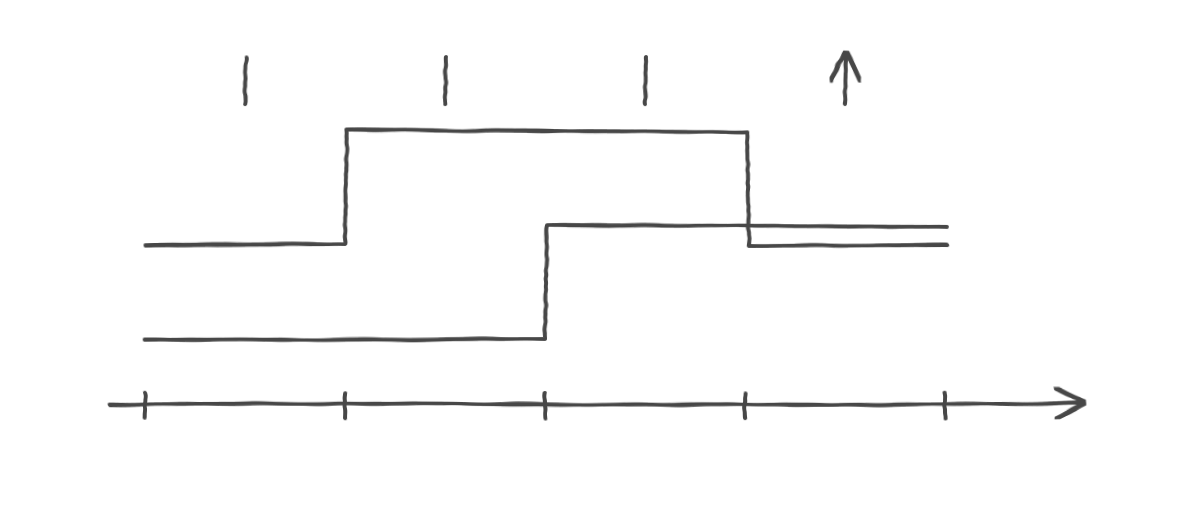
\includegraphics[width=0.92\linewidth]{032-gray-code-pencil.png}

\small Upper trace: \textbf{A}.\quad Lower trace: \textbf{B}.\quad
Samples: \textbf{00 \(\rightarrow\) 01 \(\rightarrow\) 11
\(\rightarrow\) 10 \(\rightarrow\) 00}.\quad Four valid clockwise edges.
\end{center}

\textit{Alternative text: phase B rises, phase A rises, phase B falls, then
phase A falls, producing the sampled masks 00, 01, 11, 10, 00 and four
clockwise edge decisions. Reverse traversal reports counterclockwise.}

Before power, predict the TP-A and TP-B levels for one slow traversal.\\[8pt]
\blank{5.8in}

\section{Decoder contract}

\begin{tabularx}{\linewidth}{@{}l X@{}}
\toprule
Observation & Deterministic result\\
\midrule
valid clockwise edge & \texttt{delta = +1}; increment position\\
valid counterclockwise edge & \texttt{delta = -1}; decrement position\\
same phase & zero delta; preserve position and invalid count\\
two-bit jump & zero delta; increment invalid count; adopt new baseline\\
position limit & hold at \texttt{INT32\_MIN/MAX}; report saturation\\
\bottomrule
\end{tabularx}

\texttt{reversed} exchanges the reported signs. Bounce reversals are decoded
literally; the component does not guess a detent. The invalid-transition count
saturates at 65,535. Position saturates at its signed 32-bit limits and never
wraps. \texttt{resetPosition()} changes only accumulated position and clears
position saturation; it preserves the current hardware baseline.

Initialization validates distinct Mega digital pins before claims, acquires A
then B, configures the selected pull, and reads A then B exactly once to set a
movement-free baseline. Each update again reads A once and then B once.

\section{Lifecycle and failure evidence}

If B acquisition or configuration fails, initialization rolls A back.
Repeated successful initialization performs no new hardware work. Shutdown
releases B then A, is idempotent, and retains count evidence while the
snapshot status becomes \texttt{NotInitialized}. Destruction follows the same
cleanup. Copy and move operations are prohibited.

\begin{tabularx}{\linewidth}{@{}X X@{}}
\toprule
Evidence question & Required proof\\
\midrule
Did ownership succeed? & ready indication only after both phase inputs initialize\\
Did decoding succeed? & TP sequence agrees with delta and position nibble\\
Was a jump rejected? & unchanged position plus incremented count and red pulse\\
Did shutdown become safe? & RGB/nibble inactive and both input modes released\\
\bottomrule
\end{tabularx}

An inactive LED does not prove input release. Record acquisition and
post-shutdown input-mode evidence separately.

\section{Narrative Mega example}

\begin{lstlisting}[style=adkcpp]
observeEncoder();
decideEncoderEvidence();
presentEncoderEvidence();
\end{lstlisting}

Setup acquires phase inputs, the separate button, nibble LEDs, and RGB
indicator; configures every output inactive; initializes the decoder; then
shows ready. The loop observes exactly one phase pair, decides from one stable
snapshot, and presents its low nibble and diagnostic state.

\section{Predict, observe, interpret}

\begin{enumerate}
  \item Predict the complete TP-A/TP-B sequence before applying USB power.
  \item Rotate slowly through one full electrical sequence. Observe TP-A and
        TP-B, then record four signed edges independent of mechanical detents.
  \item Compare the electrical sequence, low position nibble, and valid-edge
        pulse. Interpret agreement as decoder evidence.
  \item Reverse direction and deliberately include a small bounce reversal.
        Predict literal opposing edges rather than hidden filtering.
  \item Use only an unpowered, pre-inspected contact fixture to arrange a safe
        two-bit jump. Predict unchanged position, one invalid increment, and a
        red pulse after power is restored.
  \item Invoke shutdown separately. Record inactive displays and input
        release, then remove USB power.
\end{enumerate}

\section{Diagnosis and stop conditions}

\begin{tabularx}{\linewidth}{@{}X X@{}}
\toprule
Observation & Action and interpretation\\
\midrule
count direction reversed & verify A/B identity; use configuration reversal only intentionally\\
two bits change together & inspect contacts and sampling; expect invalid evidence\\
LED count disagrees with TP sequence & stop and inspect mapping before proceeding\\
position changes on an invalid jump & software evidence has failed; do not accept\\
hot part, resets, unstable or out-of-rail TP & remove USB immediately\\
unidentified module contact & remain unpowered until primary evidence identifies it\\
\bottomrule
\end{tabularx}

Never move jumpers while powered. Software shutdown is lifecycle behavior, not
an emergency stop; remove USB power for any unsafe or unexplained condition.

\section{Open hardware acceptance record}

\begin{tabularx}{\linewidth}{@{}l X l X@{}}
\toprule
Board/revision & \blank{1.4in} & Commit & \blank{1.25in}\\
Encoder markings & \blank{1.4in} & Pin source & \blank{1.25in}\\
Supply/instrument & \blank{1.4in} & Tool versions & \blank{1.25in}\\
Operator/date & \blank{1.4in} & Deviations & \blank{1.25in}\\
\bottomrule
\end{tabularx}

\begin{itemize}
  \item[\checkbox] unpowered identity, continuity, polarity, and resistor check;
  \item[\checkbox] acquisition prediction, observation, and interpretation;
  \item[\checkbox] both direction sequences and all four starting phases;
  \item[\checkbox] repeated state, bounce reversal, invalid jump, and recovery;
  \item[\checkbox] TP evidence and LED presentation compared independently;
  \item[\checkbox] shutdown input release, reset, and power removal recorded.
\end{itemize}

Prediction: \blank{5.8in}\\[8pt]
Observation: \blank{5.7in}\\[8pt]
Interpretation and limits: \blank{4.9in}

\section{Exercises}

\begin{enumerate}
  \item Starting at 11, list the next masks and deltas for one reverse cycle.
  \item Explain why adopting the new phase after an invalid jump enables
        recovery without inventing movement.
  \item Predict the nibble at positions \(-1\), 0, 7, 15, and 16.
  \item Design a trace that distinguishes a repeated sample from contact bounce.
  \item Explain why the separate switch belongs to \texttt{Button}, not the
        quadrature decoder.
\end{enumerate}

\section{Reproduce the software evidence}

\begin{lstlisting}[style=adkcpp]
make host-test
make host-test-exceptions
make arduino-Lesson032QuadratureEncoder
make size-check
make lessons
make lessons-check
make site-check
make hardware-card LESSON=032 BOARD=mega2560
\end{lstlisting}

Tests cover all starting phases, directions, reversal, partial turns, bounce,
repeated states, every invalid jump and recovery, both saturations, reset,
exact read order, transactional failures, lifecycle, traits, and replay.
Compilation and deterministic tests are software evidence, not a physical
module acceptance result.

\section{Reference trail}

\begin{itemize}
  \item ADK \texttt{quadrature\_encoder.h}, focused tests, and canonical
        Lesson 032 sketch;
  \item ADK Lessons 031--033 design record and authorized Elegoo family ledger;
  \item Arduino Mega 2560 Rev3 datasheet for the exact board profile.
\end{itemize}

The searchable HTML reference is the primary accessible route. This printable
PDF uses real text, headings, lists, and a monochrome timing drawing but does
not claim PDF/UA conformance.

\end{document}
